\documentclass[journal,10pt,twocolumn]{article}
\usepackage{graphicx, float}
\usepackage[margin=0.5in]{geometry}
\usepackage{amsmath, bm}
\usepackage{array}
\usepackage{booktabs}
\usepackage{mathtools}

\let\vec\mathbf
\newcommand{\myvec}[1]{\ensuremath{\begin{pmatrix}#1\end{pmatrix}}}
\newcommand{\mydet}[1]{\ensuremath{\begin{vmatrix}#1\end{vmatrix}}}

\title{\textbf{Optimization(1) Assignment}}
\author{Mukesh Guptha.ch}
\date{September 2022}

\begin{document}

\maketitle
\paragraph{\textbf{Problem Statement} -The function f(x)=x/2+2/x has a local minimum at .}

\section*{\large Figure}

\begin{figure}[H]
\centering
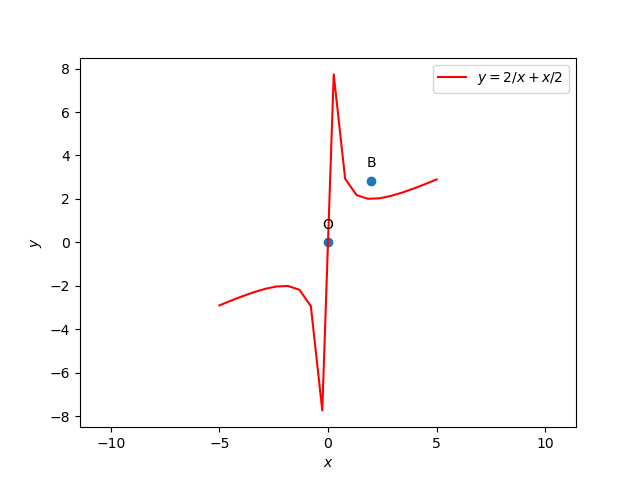
\includegraphics[width=1\columnwidth]{Figure_1.png}
\caption{Graph of f(x)}
\label{fig:triangle}
\end{figure}
\section*{\large Solution}

 
    \subsection*{\normalsize Gradient descent}
    
    
    \begin{align}
 \label{eq:vol_varx}
 f(x) = x/2+2/x\\
    f'(x) = 1/2-2/x^2
 \end{align}

we have to attain the minimum value of x/2+2/x in the interval . This can be seen in Figure f(x).Using gradient descent method we can find its minima in the interval 
\begin{equation}
        x_{n+1} = x_n - \alpha \nabla f(x_n) \\
\end{equation}
\vspace{1mm}
\begin{equation}
\implies x_{n+1}=x_n-\alpha(1/2-2/x^2)
\end{equation}

Taking $x_0=0.5,\alpha=0.001$ and precision = 0.00000001, values obtained using python are:
    

    \begin{align}
        \boxed{\text{Minima} = 2.23}\\
        \boxed{\text{Minima Point} }= 2.012340\\
    \end{align}


\end{document}
